\subsection{Generic two-port circuits}
\begin{frame}{Generic two-port circuits}
During the next experiments we will explore a few configurations of two-port circuits. The typical setup will be similar to Fig. \ref{fig:Generic_two_port} below.
\begin{figure}[hbt]
	\begin{circuitikz}
		\draw
			(0,0) node[ground] {}
			to [sinusoidal voltage source, o-o, l=$\epsilon(t)$] ++(0,2)
			to [generic, o-o, l=$Z_g$] ++(2,0)
			to [generic, o-o, l=$Z_1$] ++(2,0)
			(4,2) to [short,o-o,l_=a] ++(1,0)
			(4,2) to [generic, o-o, l=$Z_2$] ++(0,-2)
			node[ground] {}
			;
		%Description of subparts
		\draw [decorate,decoration={brace,amplitude=8pt},
					xshift=0pt, yshift=0pt]
					(2,-1) -- (-0.5,-1)
					node[black,midway,yshift=-20pt]
						{AC generator};
		\draw [decorate,decoration={brace,amplitude=8pt},
					xshift=0pt, yshift=0pt]
					(5,-1) -- (2.1,-1)
					node[black,right,yshift=-20pt]
						{Two-port circuit};	
	\end{circuitikz}
  \caption{\tiny{Generic two-port circuit setup. $Z_g$ represents the internal impedance of the AC generators, $Z_1,Z_2$ are any generic linear circuit components. The arrows $V_1$ and $V_2$ indicate where we connect  oscilloscope channels to the circuit. }}
  \label{fig:Generic_two_port}
\end{figure}

\end{frame}

\begin{frame}{Resistive voltage divider}
The simplest example of a two-port circuit is the voltage divider 			you learned in F328/F329 \cite{Walker:2008aa}. You obtain it by 			simple replacing $Z_{1,2}$ from Fig. \ref{fig:Generic_two_port} with two resistors.
	\begin{columns}
		\begin{column}{0.5\textwidth}
			\tpn{R_1}{R_2}
				\end{column}
		\begin{column}{0.5\textwidth}
		From KCL (Kirchhoff Circuit's Law):
			\begin{eqnarray}
			\Rightarrow v_1(t)=R_1 i(t)+ R_2 i(t)\\
			\Rightarrow i(t)=\frac{v_1(t)}{R_1+R_2}
			\label{eq:voltagediv_i}
  			\end{eqnarray}
		The voltage drop measured in channel 2 is given by
		\begin{equation}
  			v_2(t)=R_2 i(t)=\frac{R_2}{R_1+R_2}v_1(t)
  			\label{eq:voltagediv_v2}
		\end{equation}
		
		\end{column}
	\end{columns}
\end{frame}

\begin{frame}{Resistive voltage divider}
Based on Eq. \ref{eq:voltagediv_v2}, it is obvious now why such a circuit is called the voltage divider; the voltage measured on the \textbf{output port} of the circuit ($v_2$) is a fraction of the \textbf{input port} voltage ($v_1$).
	\begin{columns}
		\begin{column}{0.4\textwidth}
			\tpn{R_1}{R_2}
		\end{column}
		\begin{column}{0.6\textwidth}
		Using Eqs. \ref{eq:voltagediv_i} and \ref{eq:voltagediv_v2} one can now define the \textbf{frequency response} of the resistive voltage divider. For a given sinusoidal input, $v_1(t)=V_1\sin(\omega t)$, the output voltage will be given by 
\begin{equation}
  v_2(t)=\frac{R_2}{R_1+R_2}V_1\sin(\omega t)
  \label{eq:voltagediv_v2_freq}
\end{equation}
From Eq. \ref{eq:voltagediv_v2_freq} it is clear that the output voltage is \textbf{in-phase} with the input voltage but with a different amplitude.

		\end{column}
	\end{columns}
\end{frame}

\begin{frame}{Resistive voltage divider}
One can then define an output voltage $v_2(t)=V_2\sin(\omega t)$, where the amplitude $V_2=\frac{R_2}{R_1+R_2}V_1$. We now define a important quantity:
\begin{definition}
The response function of the two-port circuit network $H(\omega)$ is input-output relation $H(\omega)\equiv\frac{V_2(\omega)}{V_1(\omega)}$.
\end{definition}
Note however that although we included an explicit frequency dependence on the $H(\omega)$, in the trivial case of the resistive voltage divider $H=R_2/(R_1+R_2)$ does not depend on frequency. That simply reflects the fact that the voltage drop in a resistor is proportional to the current flowing through it.\\ In the laboratory it means that regardless of the AC generator frequency, the ratio of the voltage amplitudes measured in channels 1,2 will always be given by  $R_2/(R_1+R_2)$.
%		\begin{columns}
%			\begin{column}{0.5\textwidth}
%				\tpn{R_1}{R_2}
%			\end{column}
%			\begin{column}{0.5\textwidth}
%			
%			\end{column}
%		\end{columns}
\end{frame}

\begin{frame}{Resistive voltage divider: Numerical example}

\end{frame}

\subsection{RC voltage divider - Filters}

\begin{frame}{RC voltage divider}
We can try to apply the same principles used in the resistive voltage divider to a slightly more complex one, involving both a resistor and a capacitor. You shold also have learned about this circuit in F328/F329 \cite{Walker:2008aa}. You obtain it by 			simple replacing $Z_{1,2}$ from Fig. \ref{fig:Generic_two_port} with a capacitor and a resistor.
	\begin{columns}
		\begin{column}{0.5\textwidth}
			\tpn{R}{C}
			\tpn{C}{R}
				\end{column}
		\begin{column}{0.5\textwidth}
		From KCL (Kirchhoff Circuit's Law):
			\begin{equation}
			\Rightarrow v_1(t)=R i(t)+  q(t)/C
			\label{eq:rc_1}
  			\end{equation}
  			In contrast with the resistive divider (Eq. \ref{eq:voltagediv_i}), Eq. \ref{eq:rc_1} is an ordinary differential equation (ODE). Note that either circuit shown in the left follows the same equation. The difference is the voltage drop measured in channel 2 which will be given by
		\begin{eqnarray}
		     v_2(t)=q(t)/C\label{eq:rc_v2c}\\
		     v_2(t)=R i(t)
  			\label{eq:rc_v2r}
		\end{eqnarray}
		
		\end{column}
	\end{columns}
\end{frame}

\begin{frame}{RC voltage divider}
In order to Eqs. \ref{eq:rc_v2c},\ref{eq:rc_v2r} be useful, one must solve the ODE \ref{eq:rc_1}. It is a inhomogeneous ODE where the dependent variable is the charge $q(t)$. We can decompose its solution in two parts, $q(t)=q_h(t)+q_p(t)$, where $q_h(t)=q_0 \exp(-t/\tau)$ is the solution of the homogenous equation ($v_1=0$) and $q_p(t)$ is a particular solution which depends on the explicit form of the driving term $v_1(t)$. After the initial transients $q_h(t)$ decays and \textbf{the only important contribution is due to} $q_p(t)$. This is also called the \textbf{steady-state}.

For $v_1(t)=V_1\cos(\omega t)$ the solution is given by, 
\begin{equation}
i_p(t)=\frac{\omega C V_1 }{1+\omega^2 R^2 C^2}(\omega R C\cos(\omega t)-\sin(\omega t))=\frac{\omega C V_1 }{\sqrt{1+\omega^2 R^2 C^2}}\cos(\omega t +\phi)
\label{eq:rc_solpart}
\end{equation}
where $\phi=\tan^{-1}(\frac{1}{\omega R C})$. With Eq. \ref{eq:rc_solpart} in hand we may be tempted to proceed similarly to the resistive divider in order to derive the transfer function $H(\omega)$. Using Eqs. \ref{eq:rc_v2c},\ref{eq:rc_v2r} we obtain,
\begin{eqnarray}
v_2^{(C)}(t)=\frac{-1}{\sqrt{1+\omega^2 R^2 C^2}} V_1 \sin(\omega t +\phi) \label{eq:rc_v2final_c}\\
v_2^{(R)}(t)=\frac{\omega R C }{\sqrt{1+\omega^2 R^2 C^2}} V_1 \cos(\omega t +\phi) \label{eq:rc_v2final_r}
\end{eqnarray}

\end{frame}

\begin{frame}{RC voltage divider}
From Eq.\ref{eq:rc_v2final_c} we learn a lot about how the circuit respond to a sinusoidal excitation. In Figs. \ref{fig:bodepa_lin},\ref{fig:bodepa_log} below we plot them ($v_2^{(R)}$) in the so-called \textbf{Bode Diagrams}. Note the extra information avaliable in the $\log$ version!
	\begin{columns}
		\begin{column}{0.5\textwidth}
			\begin{figure}
  			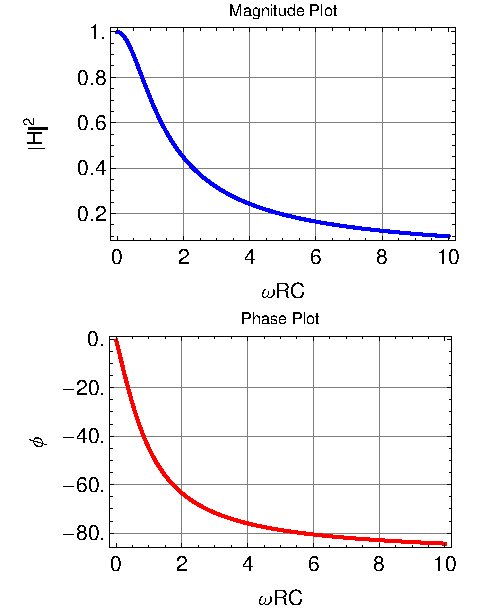
\includegraphics[width=0.7\textwidth]{bodepb_lin.pdf}
  			\caption{Linear Bode plots, $|H|^2=\frac{1}{1+\omega^2 R^2 C^2},\phi=tan^{-1}(1/\omega RC)$}
  			\label{fig:bodepa_lin}
			\end{figure}
		\end{column}
		\begin{column}{0.5\textwidth}
			\begin{figure}
  			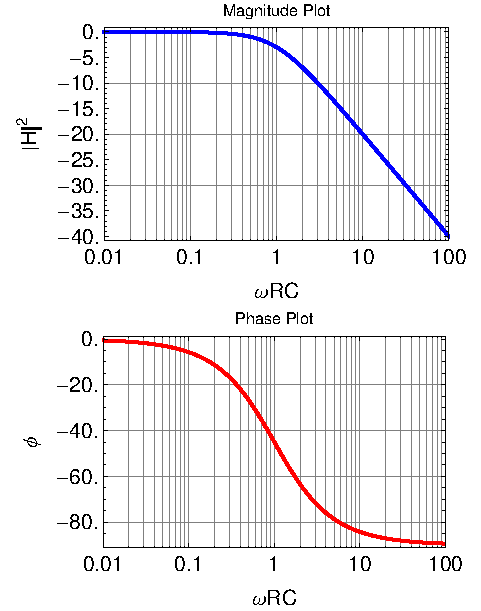
\includegraphics[width=0.7\textwidth]{bodepb_log.pdf}
  			\caption{Log Bode plots, $|H|^2=\frac{1}{1+\omega^2 R^2 C^2},\phi=tan^{-1}(1/\omega RC)$}
  			\label{fig:bodepa_log}
			\end{figure}
		\end{column}
	\end{columns}
\end{frame}

\begin{frame}{RC voltage divider}
From Eq.\ref{eq:rc_v2final_r} we learn a lot about how the circuit respond to a sinusoidal excitation. In Figs. \ref{fig:bodepa_lin},\ref{fig:bodepa_log} below we plot them ($v_2^{(C)}$) in the so-called \textbf{Bode Diagrams}. Note the extra information avaliable in the $\log$ version!
	\begin{columns}
		\begin{column}{0.5\textwidth}
			\begin{figure}
  			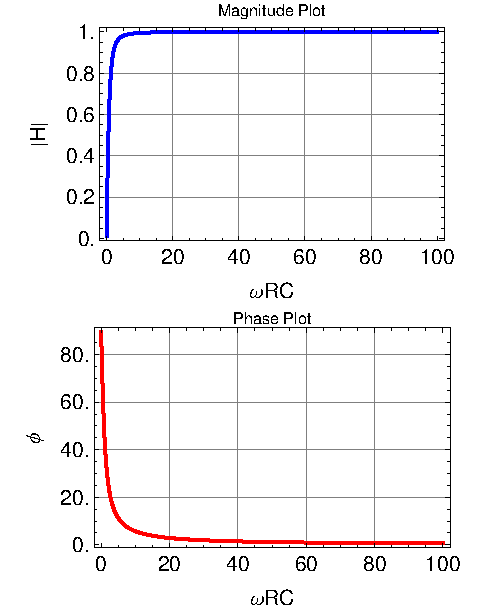
\includegraphics[width=0.7\textwidth]{bodepa_lin.pdf}
  			\caption{Linear Bode plots, $|H|^2=\frac{\omega R C}{1+\omega^2 R^2 C^2},\phi=tan^{-1}(1/\omega RC)$}
  			\label{fig:bodepa_lin}
			\end{figure}
		\end{column}
		\begin{column}{0.5\textwidth}
			\begin{figure}
  			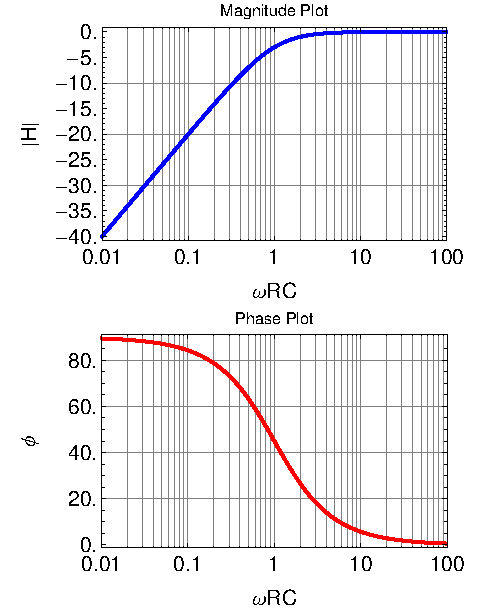
\includegraphics[width=0.7\textwidth]{bodepa_log.pdf}
  			\caption{Log Bode plots, $|H|^2=\frac{\omega R C}{1+\omega^2 R^2 C^2},\phi=tan^{-1}(1/\omega RC)$}
  			\label{fig:bodepa_log}
			\end{figure}
		\end{column}
	\end{columns}
\end{frame}
\subsection{RLC circuit}

\begin{frame}{RLC circuit}
	\begin{columns}
		\begin{column}{0.5\textwidth}
			\begin{circuitikz}[scale=1]
		\node (Xi) at (0.7,0.7) {$V_1$};
		\node (Xf) at (5.7,0.7) {$V_2$};
		\draw [semithick,->] (Xi) -- (0.1,0.1);
		\draw [semithick,->] (Xf) -- (5.1,0.1);
		\draw
			to [inductor, o-o, l_=L] ++(2,0)
			to [capacitor, o-o, l_=C] ++(2,0)
			(4,0) to [short,o-o] ++(1,0)
			(4,0) to [resistor, o-o, l=R] ++(0,-2)
			node[ground] {}
			;
\end{circuitikz}

		\end{column}
		\begin{column}{0.5\textwidth}
		The KCL equation now reads
\begin{eqnarray}
v_1(t)=L \frac{di}{dt} + q(t)/C +R i(t)\label{eq:rlc_kcl1}\\
\Rightarrow \frac{1}{L}\frac{dv_1}{dt}=\frac{d^2i}{dt^2} + \frac{R}{L} \frac{di}{dt} + \frac{1}{LC}i
\label{eq:rlc_kcl2}
  \end{eqnarray}
  Of course we could repeat the process of attempting to find a solution of the form $i(t)=i_0 \cos(\omega t+\phi)$ for a given $v_1(t)=V_1 \cos(\omega t)$. That would work perfectly and you can work out the result.
  
We want however a more powerful method for looking at such circuits!
		\end{column}
	\end{columns}
\end{frame}

\begin{frame}{Complex numbers \& Trigonometric functions}
\begin{figure}[hbt]
  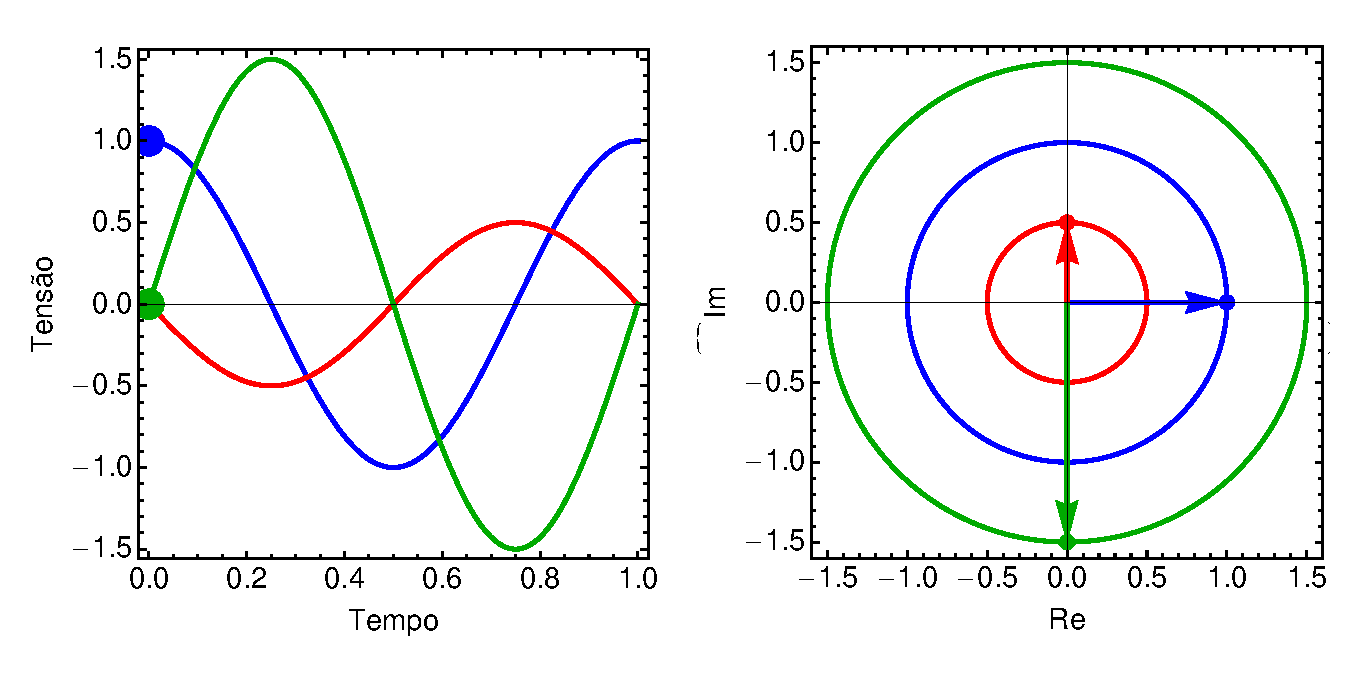
\includegraphics[width=\textwidth]{fasor0.pdf}
  \caption{Phasor at t=0}
\end{figure}
\end{frame}

\begin{frame}{Complex numbers \& Trigonometric functions}
\begin{figure}[hbt]
  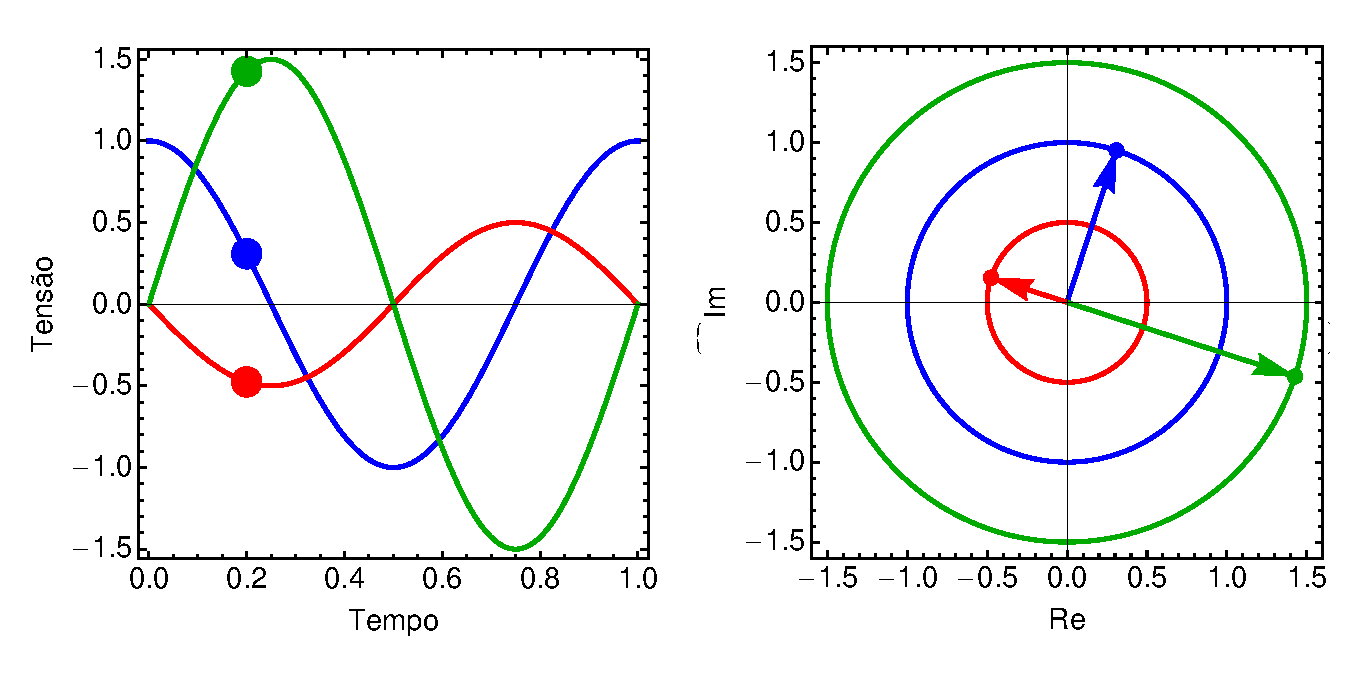
\includegraphics[width=\textwidth]{fasor0p2.pdf}
  \caption{Phasor at t=0.2}
\end{figure}

\end{frame}

\begin{frame}{Complex numbers \& Trigonometric functions}
The connection between these things lies on the identity
\begin{equation}
  \exp(ix)=\cos(x)+j\sin(x)
\end{equation}


\end{frame}
\begin{frame}{Complex numbers \& Trigonometric functions}
\begin{proof}
Let's define $f(x)=\cos(x)+j\sin(x)$. Therefore $f'(x)=-\sin(x)+j\cos(x)=j[\cos(x)-\frac{1}{j}\sin(x)]$. However $j^2\equiv -1$, $\Rightarrow f'(x)=j[\cos(x)+{j}\sin(x)]=j f(x)\Rightarrow f(x)=\exp(j x)$
\end{proof}

\end{frame}




%(0,0) node[ground] {} (0,0)
%to [sinusoidal voltage source, o-o, l=$\epsilon(t)$] ++(0,2)
%to [R, o-o, l=$R_g$] ++(2,0)
%to [generic, o-o, l=$Z_1$] ++(2,0)
%to [generic, o-o, l=$Z_2$] --(0,2)
%;
